\def\mytitle{Implementation of 8 Input comparator}
\def\mykeywords{}
\def\myauthor{A.Hari Venkateswarlu }
\def\contact{hariannam99@gmail.com}
\def\mymodule{Future Wireless Communication(FWC22058)}
\documentclass[10pt, a4paper]{article}
\usepackage[a4paper,outer=1.5cm,inner=1.5cm,top=1.75cm,bottom=1.5cm]{geometry}
\twocolumn
\usepackage{graphicx}
\usepackage{amsmath}
\usepackage{circuitikz}
\usetikzlibrary{calc}
\graphicspath{{./images/}}
%colour our links, remove weird boxes
\usepackage[colorlinks,linkcolor={black},citecolor={blue!80!black},urlcolor={blue!80!black}]{hyperref}
\usetikzlibrary{arrows,shapes.gates.logic.US,shapes.gates.logic.IEC,calc}
%Stop indentation on new paragraphs
\usepackage[parfill]{parskip}
%% Arial-like font
\usepackage{lmodern}
\renewcommand*\familydefault{\sfdefault}
%Napier logo top right
\usepackage{watermark}
%Lorem Ipusm dolor please don't leave any in you final report ;)
\usepackage{lipsum}
\usepackage{xcolor}
\usepackage{listings}
\usepackage{float}
\usepackage{titlesec}
\usepackage{amsmath}
\usepackage{algorithm2e}
\usepackage{circuitikz}

\titlespacing{\subsection}{0pt}{\parskip}{-3pt}
\titlespacing{\subsubsection}{0pt}{\parskip}{-\parskip}
\titlespacing{\paragraph}{0pt}{\parskip}{\parskip}
\newcommand{\figuremacro}[5]{
    \begin{figure}[#1]
        \centering
        \includegraphics[width=#5\columnwidth]{#2}
        \caption[#3]{\textbf{#3}#4}
        \label{figure:#2}
    \end{figure}
}

\lstset{
frame=single, 
breaklines=true,
columns=fullflexible
}

\thiswatermark{\centering \put(0,-90.0){
\includegraphics[scale=0.05]{iith_logo.png}} }
\title{\mytitle}
\author{\myauthor\hspace{1em}\\\contact\\IITH\hspace{0.5em}-\hspace{0.5em}\mymodule}
\date{}
\hypersetup{pdfauthor=\myauthor,pdftitle=\mytitle,pdfkeywords=\mykeywords}
\sloppy
% #######################################
% ########### START FROM HERE ###########
% #######################################
\usepackage{tabularx}
\begin{document}
	\maketitle
	\tableofcontents
	\begin{abstract}
	    %Replace the lipsum command with actual text 
Design a sequential circuit that take(A3 A2 A1 A0 ) and (B3 B2 B1 B0) compares both A and B.The output should be 1.A$<$B, 2.A$>$B, 3.A=B on seven segment display.
	\end{abstract}
    \section{Introduction}
    A comparator is an electronic circuit, which compares the two inputs that are applied to it and produces an output. The output value of the comparator indicates which of the inputs is greater or lesser. Please note that comparator falls under non-linear applications of ICs.
	\section{Components}
	
\begin{table}[htbp]
 \begin{center}
    \begin{tabular}{|l|c|c|c|c|c|c} \hline \textbf{Component}
  & \textbf{value} & \textbf{quantity} \\
 \hline
Resistor & 220 ohm & 1 \\ \hline
Arduino & UNO & 1 \\ \hline
decoder & 7447 & 1  \\ \hline
Jumper wires & M-M & 20\\ \hline
sevensegment display &  & 1 \\ \hline
Bread board &  & 1 \\ \hline
\end{tabular}   
\end{center}
\caption{\label{table:table} }
\end{table}
	\section{Hardware}
	\textbf{3.1}
    Connection between the sevensegment display and 7447 IC in Figure 1 using Table 2.
    \begin{center}
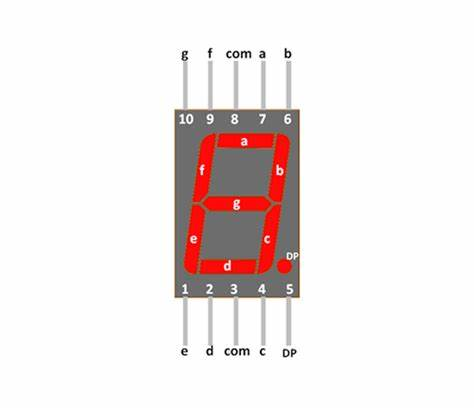
\includegraphics[scale=.20]{sevenseg.jpg}
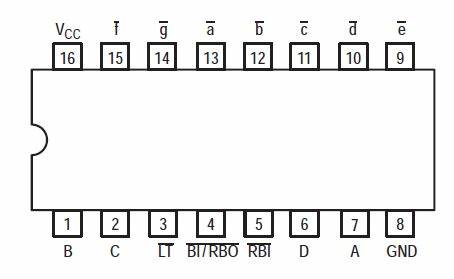
\includegraphics[scale=.20]{7447ic.jpg}
\end{center}
\centering\textbf\ Figure 1:Sevensegment and 7447 IC.
	\begin{table}[htbp]
    \begin{center}
    \begin{tabular}{|l|c|c|c|c|c|c|c|c} \hline \textbf{7447}
  & a' & b' & c' & d' & e' & f' & g' \\
 \hline
\textbf{Display} & a & b & c & d & e & f & g \\ \hline
\end{tabular}   
\end{center}
\caption{\label{table:dummytable} }
\end{table}
\\	\textbf{3.2}
	connection of lower pins of 7447 IC to the Arduino according to Table 3 and connecting VCC,GND of IC to 5V,GND of Arduino respectively.
		\begin{table}[htbp]
    \begin{center}
    \begin{tabular}{|l|c|c|c|c|c|c|c|c} \hline \textbf{7447}
  & D & C & B & A \\
 \hline
\textbf{Arduino} & 10 & 11 & 12& 13\\ \hline
\end{tabular}   
\end{center}
\caption{\label{table:dummytable} }
\end{table}
\\\textbf{3.3}
Finally, give connections to the arduino and inputs based on table 4.
	\begin{table}[htbp]
    \begin{center}
    \begin{tabular}{|l|c|c|c|c|c|c|c|c|c|} \hline 
 
\textbf{Input} & A0 & A1 & A2 & A3 & B0 & B1 & B2&B3 \\ \hline
\textbf{Arduino} & 2 & 3 & 4 & 5& 6 & 7 & 8 & 9\\ \hline
\end{tabular}   
\end{center}
\caption{\label{table:dummytable} }
\end{table}
\section{Implementation}
\textbf{4.1}
By making Logic circuit based on comparator logic we get the circuit as in figure 2.

\textbf{4.2}
The code below realizes the 8 input comparator.
\begin{lstlisting}
https://github.com/hari1847/hari/tree/main/assembly/codes
\end{lstlisting}



 \begin{center}
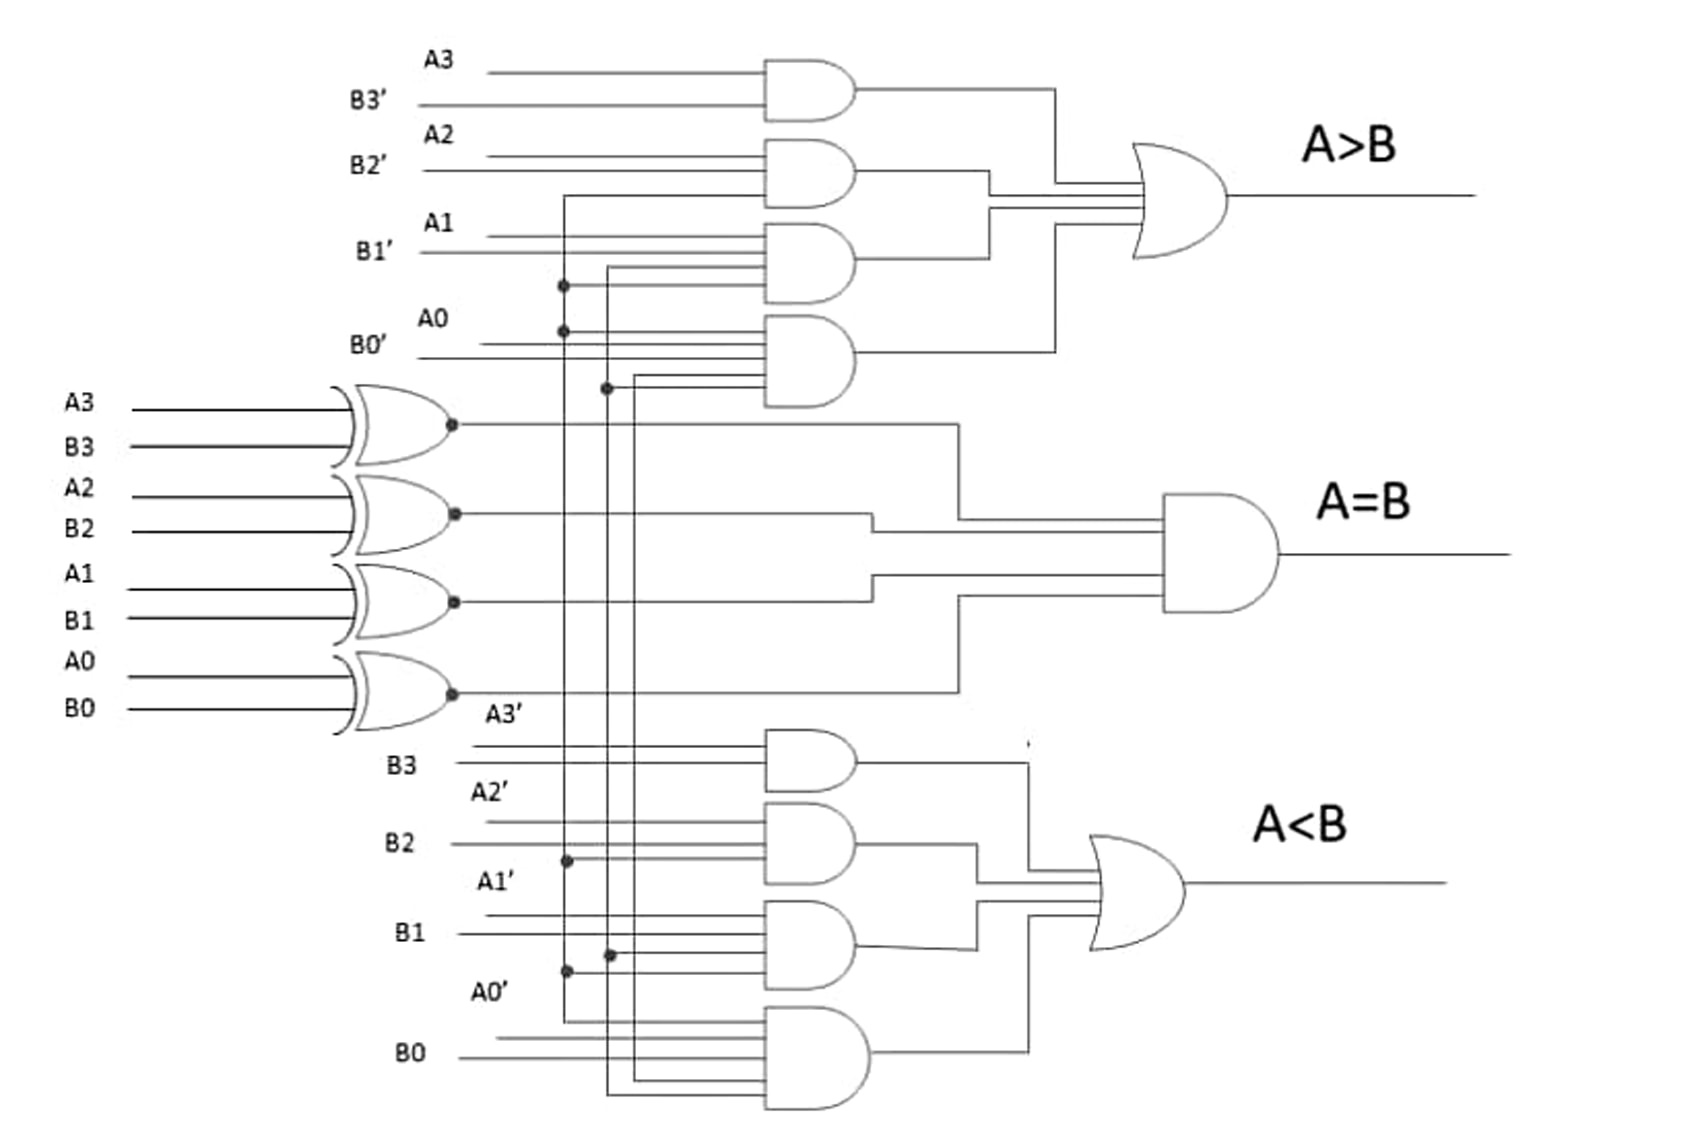
\includegraphics[scale=.10]{circuit.jpeg}

\end{center}
\begin{center}
    Figure 2
\end{center}

\end{document}